In most programming languages the first program people write is the so called ``Hello World'' program.

The main idea is to show \code{Hello World} to the user.

\vspace{0.5em}

So let's create this \code{hello-world.tau} file!

\subsection{Structure}
A tau program is divided into two different parts: The head and the body. 
The head contains all the necessary base information whilst the body contains the state machine.

\subsubsection{The head}
In the head we can define what the Turing Machine needs:
\begin{enumerate}
    \item The different symbols the Turing Machine can read/write on the tape
    \item The blank symbol on the tape
    \item The state that should be the state that the Turing Machine starts with
    \item The state where the Turing Machine should end
    \item If something should be on the tape before the machine runs the tape also needs to be specified
\end{enumerate}

So let's define the ones we need:
\begin{verbatim}
    symbols = 0, Hello, World
    blank = 0

    start = ?
    end = ?
\end{verbatim}

(The contents of \code{start} and \code{end} currently contain a \code{?} as we do not currently know what should be put in here.)

So what can we see?

\begin{itemize}
    \item Every single statement we define has the structure: 
    \begin{center}
        \code{<name> = <value>}
    \end{center}
    \item \code{symbols} contains more than one element and is therefore separated with \code{,}.
    \item The different statements do not end with any specific character (like \code{;} in C-style languages).
          The end is being inferred.
\end{itemize}

We also define one extra symbol with \code{0}, which is our blank element. This element is by default on the tape. 
We could also specify that \code{Hello} is the blank element, but this isn't done as it does not make sense in this context.

We will later on define the starting state as \code{HELLO} as it is the state that writes \code{Hello} onto the tape 
and the end state as \code{HALT} as it will halt the Turing Machine. This means that the head will now look like this:
\begin{verbatim}
    symbols = 0, Hello, World
    blank = 0
    
    start = HELLO
    end = HALT
\end{verbatim}

Now to end the head and start the body we can write any number of \code{-} as a delimitor. For example something like this: \code{----}.

\subsubsection{The body}
The body contains the state machine. This state machine is the heart of the Turing Machine. 
So let's visualize how the state machine should look like before we actually implement it:

\begin{center}
    \begin{tikzpicture}[->, % makes the edges directed
        >=stealth, % makes the arrow heads bold
        node distance=4cm, % specifies the minimum distance between two nodes. Change if necessary.
        every state/.style={fill=gray!10}, % sets the properties for each ’state’ node
        initial text=$ $, % sets the text that appears on the start arrow
        current state/.style={
            fill=gray!40
        }]
    
        \node[state, initial] (Hello) {\code{HELLO}};
        \node[state, right of=Hello] (World) {\code{WORLD}};
        \node[state, accepting, right of=World] (Halt) {\code{HALT}};
    
        \draw (Hello) edge[above] node{\_ | Hello, R} (World);
        \draw (World) edge[above] node{\_ | World, S} (Halt);
    \end{tikzpicture}
\end{center}

Here we start with the \code{HELLO} state and for any element on the tape (The ``\code{\_}'' stands for any character on the tape) 
\code{Hello} should be written on the tape, the head on the tape should move to the right and go to the next state \code{WORLD}.

In this state for any element on the tape it should write \code{World} to the tape, the head should stay and go to the next state \code{HALT}.

As \code{HALT} is the end state, the Turing Machine stops.

\vspace{0.8em}

And now the tape should look like this:
\begin{center}
    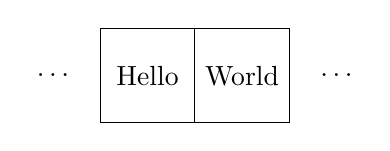
\begin{tikzpicture}[scale=1.2]
        \node at (-0.5,0.5) {$\dots$};
        \draw (0,0) rectangle (1,1);
        \draw (1,0) rectangle (2,1);
        \node at (0.5,0.5) {\code{Hello}};
        \node at (1.5,0.5) {\code{World}};

        \node at (2.5,0.5) {$\dots$};
    \end{tikzpicture}
\end{center}

This means that we can now write the states in the \code{hello-world.tau} file:
\begin{verbatim}
    HELLO {
        _ = Hello, RIGHT, WORLD
    }

    WORLD {
        _ = World, STAY, HALT
    }
\end{verbatim}

With this syntax the state name is being defined at the beginning and then the curly brackets (\code{\{\}}) contain the different rules. 
As the \code{HALT} rule doesn't do anything by itself it does not have to be defined.

Each rule is being specified with the syntax \code{<Current Symbol> = <New Symbol>, <Direction>, <Next State>}. 
As we don't care about the current element on the tape we can just use a \code{\_} to delimit that this should happen to every other Symbol that wasn't defined.

\subsubsection{Final Tau Script}
So. To put all of this together we get a script inside the \code{hello-world.tau} like this:

\begin{verbatim}
    symbols = 0, Hello, World
    blank = 0
    
    start = HELLO
    end = HALT

    ----

    HELLO {
        _ = Hello, RIGHT, WORLD
    }

    WORLD {
        _ = World, STAY, HALT
    }
\end{verbatim}

\subsection{Executing the program}
To now execute this tau script, just go to the path of the Tau binary and type in \code{./tau hello-world.tau} 
(If you have saved your \code{hello-world.tau} somewhere else, you have to specify a different path to the file)

This should now print something like this:
\begin{verbatim}
    Execution sequence:

    State: HELLO
    ..., 0, 0, 0, 0, 0, 0, 0, 0, 0, ...
                     ^
                     Hello

    State: WORLD
    ..., 0, 0, 0, Hello, 0, 0, 0, 0, 0, ...
                         ^
                         World

    State: HALT
    ..., 0, 0, 0, Hello, World, 0, 0, 0, 0, ...
\end{verbatim}

And now you have written and executed your first Tau program. Yay!

\subsection{Comments}
Comments are an essential aspect of documenting the code so that other people and your later self can understand what the code does
if it doesn't work what the intention was.

In Tau there are only single line comments. They start with a \code{\#} and end with the next Line separator (\code{\textbackslash n}).

These comments can be added anywhere and nothing inside the comment will be parsed.

\begin{verbatim}
    # This is a simple comment

    ## Comments can also contain multiple # as well

    symbols = 1 # They can also be after some other tokens
    , 2, 3 # And even though this looks awful

    # This is the same as just writing "symbols = 1,2,3"
\end{verbatim}
